\documentclass[WordOneHalf]{XDUthesis} %[Fandol]%[nologo]%[WordOneHalf]%[Fandol,nologo]%[WordOneHalf,nologo]%[WordOneHalf,Fandol,nologo]

\title{基于XDUthesis模板的论文写作样例}
\author{崔元顺}
\date{2016年05月15日}
%题目拆分:用于封面
\septitleA{基于\XDUthesis{} 模板的}%如果论文题目长度<=11中文字符只需填此项即可B项空着
\septitleB{论文写作样例}%如果论文题目长度>11中文字符, 建议拆分为10+x or 11+x 将剩余x个字符填在此处。
\class{0712**}%班级号
\schoolnumber{0712****}%学号
\major{统计学}%专业
\school{数学与统计学院}%学院
\supervisor{崔元顺}%指导老师

%\usepackage[BoldFont]{xeCJK}

\begin{document}

% 摘要
% 中文摘要
\begin{abstract}
随着近几年中国汽车保有量的持续增加,智能交通系统以及自动驾驶技术俨然已成为十分
热门的研究领域。而机动车车牌识别技术作为这两项技术的基础和关键,有着十分重要的研
究意义和应用价值。本文主要对车牌识别系统所涉及的车牌检测、车牌定位、车牌字符分割
和车牌识别四个子系统展开研究,并运用最新的深度学习技术实现一个简单的车牌识别系统。
全文工作将分为以下几点:

第一,本文首先阐述本课题的研究背景及意义,并简要介绍深度学习技术相较于传统技术的
异同;

第二,本文尝试使用Faster R-CNN技术来进行车牌检测,来克服传统方法严重依
赖手工特征和手工规则、鲁棒性差等缺点;

第三,本文尝试使用CNN 回归车牌顶点坐标的方法以实现车牌定位;

第四,车牌字符分割问题可以看做对车牌图片中的文字进行
提取的问题。本文尝试使用Class-specific Extremal Region的方法进行车牌字符分割;

第五,在图像识别领域,目前最理想的方法当属卷积神经网络(简称CNN),它有着更好的
识别准确率和更强的鲁棒性。因此本系统采用CNN 的方法进行车牌识别。

最后,本文总结了深度学习技术及其在车牌识别这一计算机视觉任务上的应用前景,并提出
对未来的展望。
\end{abstract}
\keywords{车牌检测, 车牌定位, 车牌字符分割, 车牌识别, 深度学习}

% 英文摘要
\begin{enabstract}
With the continued increase in vehicle ownership in China in recent years,
intelligent transportation system and autopilot technology has became a very
popular research field. As the foundation and key of these two technologies,
the vehicle license plate recognition technology is of great importance in both
research and application. This paper focuses on four
essential subsystem in the vehicle license plate recognition system including
detection, localization, segmentation and recognition. We implement a simple vehicle
license plate recognition systems based on the up to date deep learning
technologies. We summarize the whole work as follows:

First, we illustrates the certain necessity of the research and implementation
of this vehicle license plate recognition system by describing the background and
significance of the research.

Second, This paper will
present an approach of vehicle license plate detection based on Faster R-CNN
technology, in order to overcome the shortcomings of traditional
methods such as the dependency of hand-made features as well as the
poor robustness.

Third, in this paper, we try to localize vehicle license plate by regressing the
vertex positions using CNN.

Fourth, The vehicle
license plate segmentation problem can be viewed as the problem of detecting
characters from license plate pictures. In this paper, we try to segment license
into character by using Class-specific Extremal Region technology.

Fifth, in the field of image recognition, there is no doubt that CNN is the
state-of-art approach currently, it has a higher accuracy and a better
robustness. So we adopt the CNN for license plate recognition in our final
system.

Sixth, through the study of the technologies above, this paper implements a
simple license plate recognition system. In our recognition system, we use RCNN
for detection, CNN regression for location, CSER for character segmentation and
CNN for the final recognition, respectively.
\end{enabstract}
\enkeywords{vehicle license plate detection, vehicle license plate location,
  vehicle license character segmentation, vehicle license plate recognition,
  deep learning}

% 往PDF属性里面写下关键词信息
\makeatletter
\XDU@setpdf@keywords
%\make@abstract%
%
%\frontmatter
%\tableofcontents%
%\mainmatter
\makeatother

\maketitle

% 文章主要部分
\chapter{引言}
\section{研究背景和研究意义}
\subsection{研究背景}

自从十九世纪八十年代人类世界的第一辆汽车诞生以来,人类的生活就再也离不开汽车这种
方便的交通工具。尤其是进入21世纪以来,中国大陆地区汽车保有量快速上升,几乎到了家
家都有车的地步,一些富裕一些的家庭甚至一人一辆车。据不完全统计,在2002年左右我国
的汽车保有量在2000万辆左右,而到了2015年则增加到1.72亿辆之多,并且以每年百分之十
的速度持续增长。如此大量的汽车,在给我们带来诸多便利的同事,也增加了城市道路的
复旦和交通事故的发生率。如今,道路拥堵、违规停车、交通事故已成为每个城市管理者的
心头病。因此,各国政府也在一直不停的研究如何对车辆有效监管,提高道路利用率,避免
交通事故。在此前提下,诞生了两大热门研究方向:智能交通系统(Intelligent
Transportation System, ITS)和自动驾驶系统。这两项技术都旨在通过计算机技术来解决
交通管理等问题。而这两项技术中必不可少的一环便是进行车牌识别,即通过计算机视觉技
术,对图像(或视频)中的车牌进行准确的定位、分割和识别。

\subsection{研究意义}

从研究背景中我们可以知道,VLPR 技术在实际生活中有着十分重要且广泛的应用。下面我们
举出几个实际生活中自动车牌识别系统的典型应用:

\subsubsection{停车场的智能管理}

一般而言,在住宅小区、大型商场、车站等地方都会建设配套的停车场。而如何对进出停车
场的车辆进行管理,则是一个十分重要的问题。目前常见的有三种方式:

\begin{itemize}
\item 纯人力管理
\item 发放出入门禁卡
\item 智能的电子化管理
\end{itemize}

其中前两种方式都有着管理成本高、需要人力维护等缺点,而通过使用智能化电子管理系统,
不仅有效降低了管理、维护成本,而且可以实现无人值守式停车场。因此可以看到目前使用
智能化电子管理的停车场数量在不断增加。一般的智能化电子管理系统是在停车场的出入口
架设摄像头,自动对进出的车辆进行拍照,并对车辆的车牌号进行识别,从而对车辆进行登
记管理。

\subsubsection{停车场自动找车系统}

随着停车场越建越大,相信在若大的停车场里找寻自己的车辆是每个车主都头疼过得问题。
目前市面上出现了一项新的自动找车系统,即通过在停车场内部署的大量摄像头,对停在不
同车位的车辆进行车牌识别。车主在找车的时候,只需在终端机上输入自己车辆的车牌号,
系统就会自动找到车辆位置,并为车主提供导航。这项技术也大大方便了人们的生活、提高
了停车场的用户体验。

\subsubsection{电子警察系统}

目前的电子警察系统,通过大量安装道路路口、路段上的摄像头,对车道内的机动车驾驶行
为进行不间断自动检测和记录,并检测车辆的违法驾驶行为。而这项系统也必然少不了车牌
识别系统的帮助。可以看到,目前通过对城市道路电子警察的大量部署,可以有效对城市道
路上的车辆进行24小时的监控,很大程度上降低了交通事故的发生率。

\subsubsection{行车记录系统}

随车道路上车辆的不断增加,交通事故总是不可避免。为了方便在发生事故时进行责任认定,
许多车主都在汽车上加装了行车记录仪以记录行车情况。而如果一个行车记录仪能够自动进
行车牌识别并记录行车过程中周围的车辆信息,则无疑会大大方便车主和交警进行事故责任
认定等。

\subsubsection{自动驾驶系统}

基于人工智能技术的自动驾驶系统被认为是未来交通系统的希望之星。众所周知,人类驾驶
员在驾驶过程中难免存在疲劳、注意力分散、视角盲区等问题,从而造成了大量的交通事故。
而自动驾驶系统则无这些缺陷,因此可以在很多情况下降低交通事故的发生概率。因此许多
科技公司和研究机构都投入了大量的人力物力以进行自动驾驶技术的研究。事实上德国已经
开始尝试使用自动驾驶的卡车进行高速公路货运,以减少人力成本和交通事故。因此,车牌
识别系统作为自动驾驶系统里必不可少的一个子环节,有着十分重要的研究意义。

\begin{figure}[ht]
  \centering
  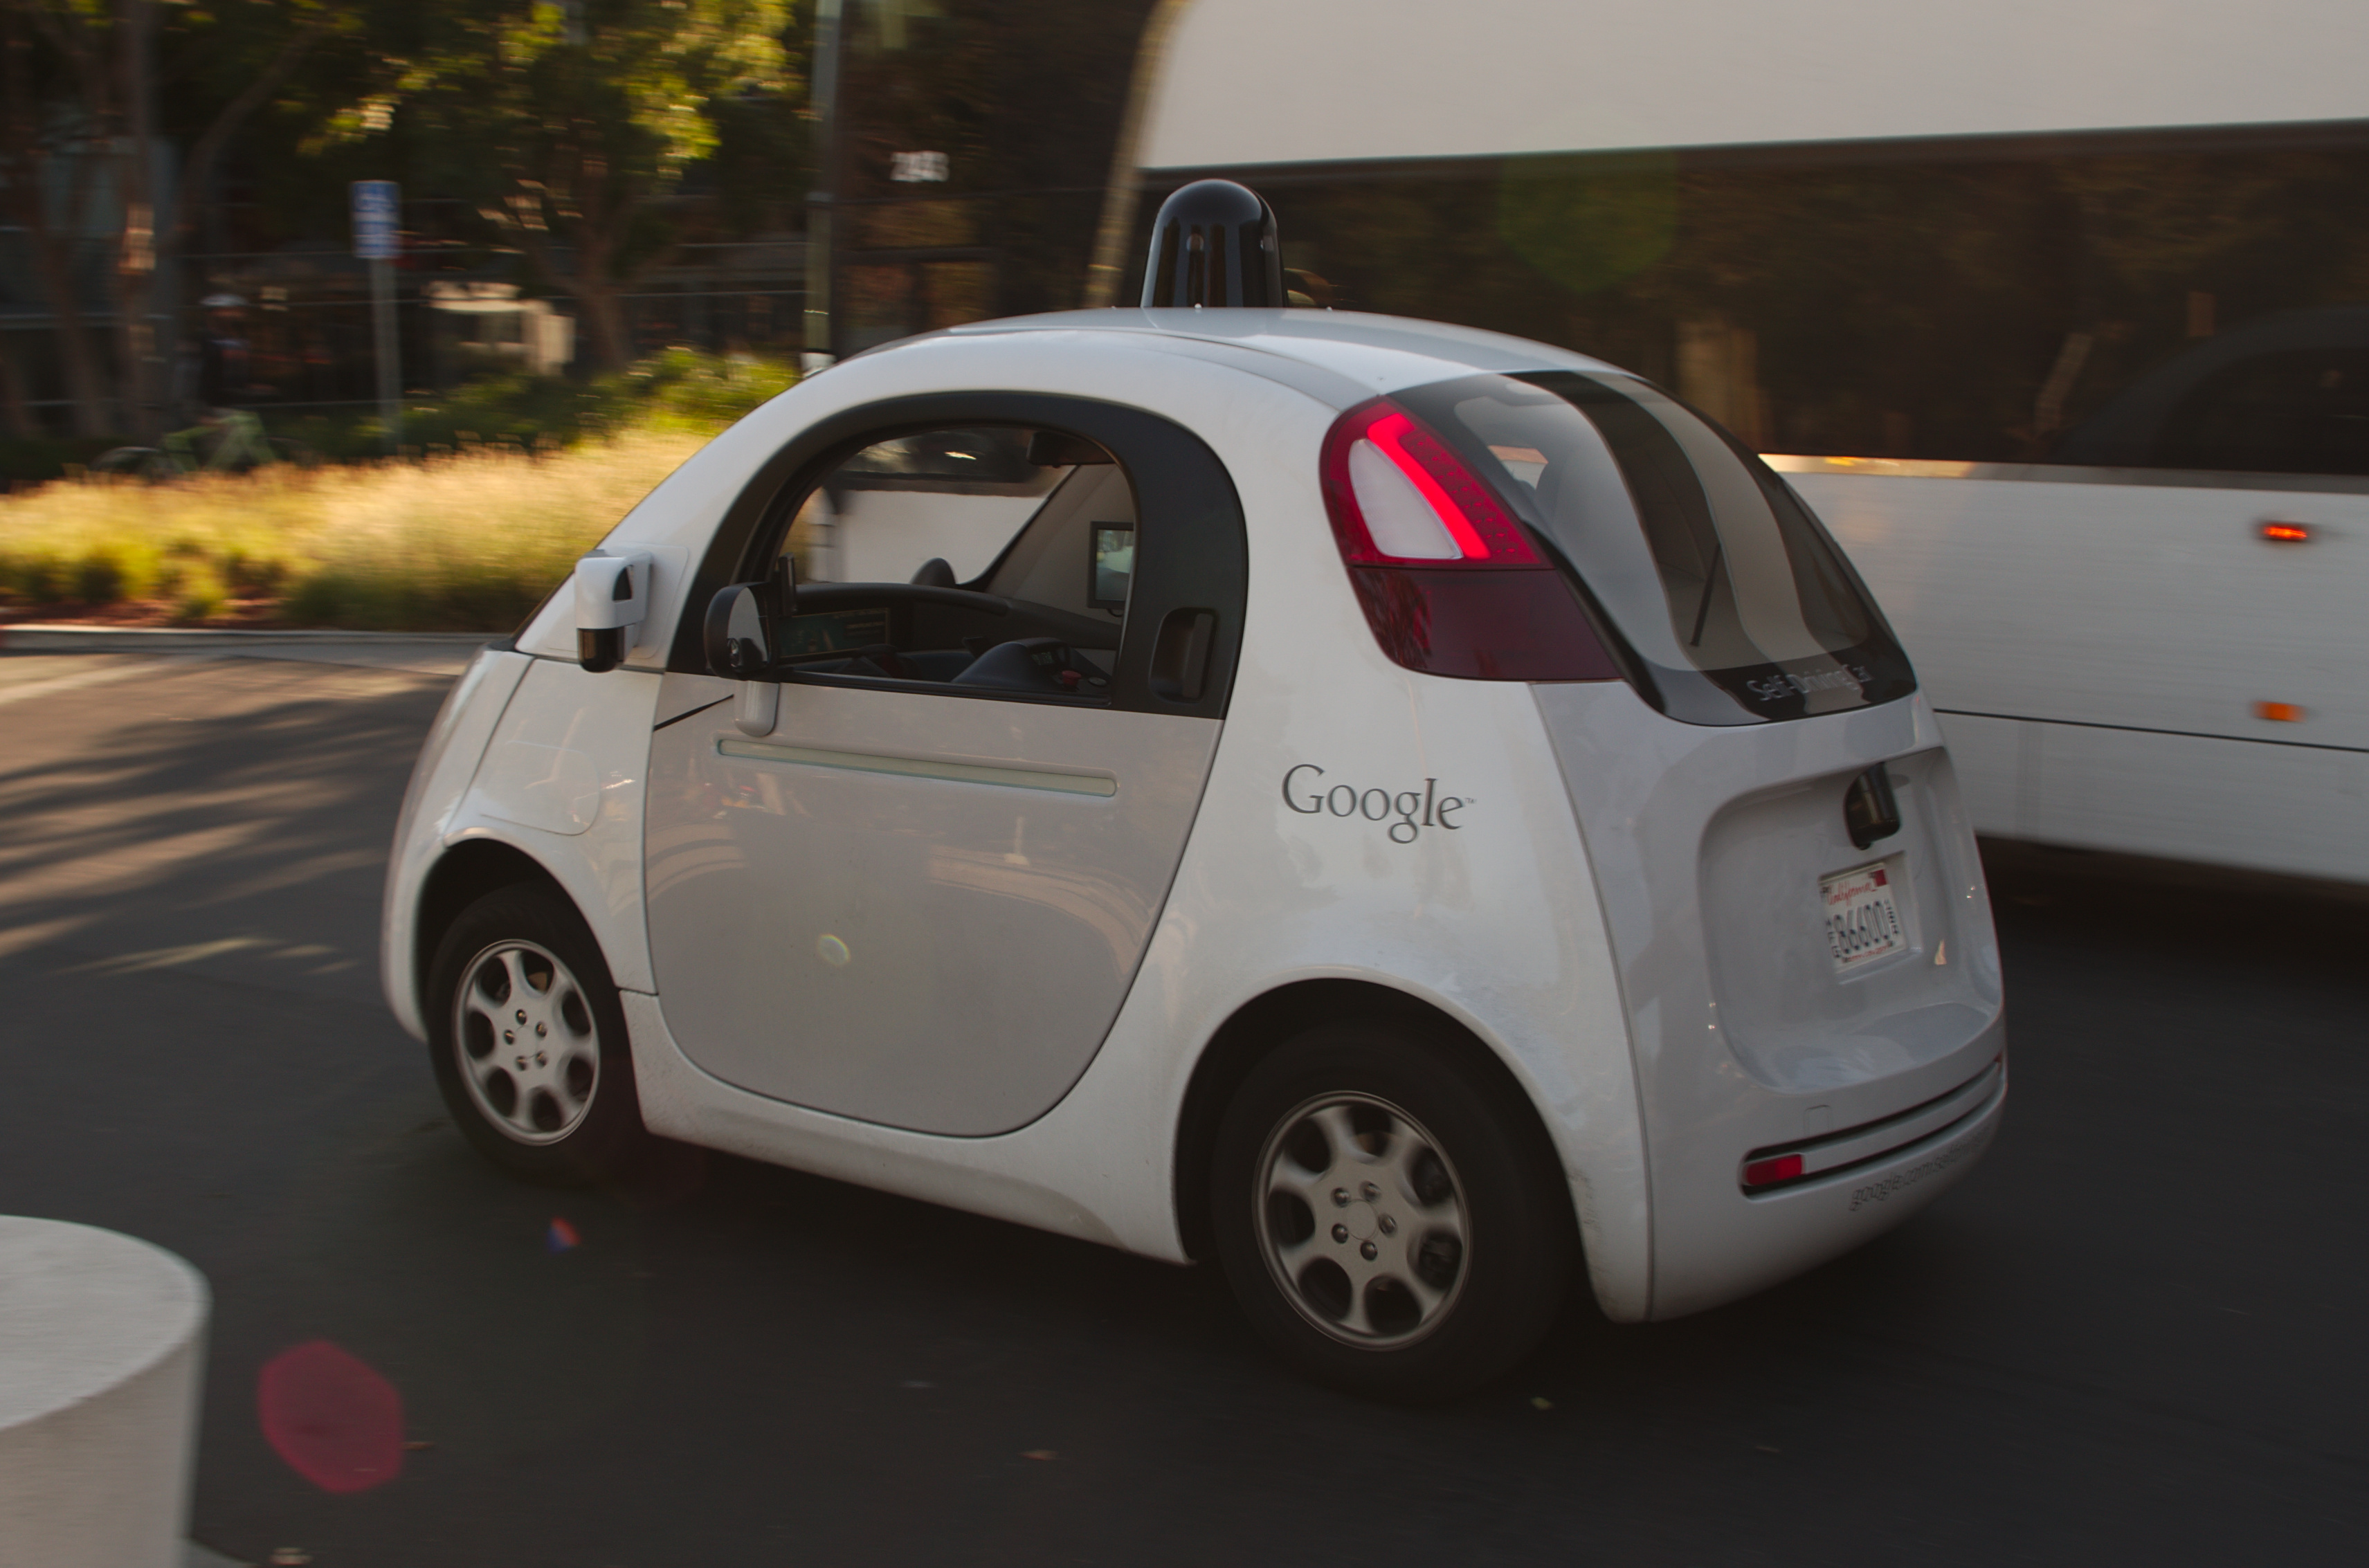
\includegraphics[width=0.8\linewidth]{./Figure/GoogleSelfDrivingCar.jpg}
  \caption{Google公司研制的无人驾驶汽车}
\end{figure}

综上所述,基于计算机视觉技术的车牌识别方法在诸多领域都有着极为广泛的应用前景和市
场价值,能够对社会和人类带来极为深远的影响。

\section{深度学习与计算机视觉}
\subsection{传统方法}

本文中提到的传统方法,是指在机器学习技术引入计算机视觉之前,人们为了解决常见的视
觉问题发明的大量基于手工特征和手工规则的方法。比较经典的,比如用于直线、曲线检测的
广义Hough变换,用于边缘检测的Sobel算子以及SIFT、SURF、HoG等图像特征。这些方法在早期的计
算机视觉任务中被大量的使用,并取得了一定的效果。比如,许多车牌检测系统使用Hough变
换对车牌的边缘进行检测从而实现车牌边缘的定位;使用二值化方法结合直方图投影进行车
牌字符分割。

由于传统的计算机视觉方法严重依赖于图像特征的选择,因此这些方法不仅需要花费大量的
精力进行特征工程,而且难以胜任一些复杂的计算机视觉任务,比如自然场景中的物体检测、
字符识别等任务。同时,即使是在一些已取得成功应用的领域,这些方法的效果也与人类视
觉系统的能力相距甚远。于是很自然的,人们就想如果手工设定的规则和特征不能很好的适
用于各种复杂计算机视觉任务,那为什么不让计算机自己从数据中学习特征和规则呢?于是
机器学习技术开始被应用于计算机视觉任务中,其中在近几年的研究中又以深度学习技术效
果最好、应用最广。

\subsection{深度学习}

所谓深度学习技术,实际上就是神经网络技术,只不过相较于传统的多层感知机等浅层神经
网络模型,深度学习中使用的网络模型层数更多(即更深)、规模更大。目前主流的深度神
经网络模型可以分为卷积神经网络CNN和递归神经网路RNN 两类。其中CNN 被广泛应用于各类
图像相关的计算机视觉任务中,而RNN 更多的应用在自然语言处理、时间序列预测等时序相
关的任务中。本文所采用的方法都是基于CNN 的,因此在此着重介绍CNN 的发展和应用。
1998年前后,Yann LeCun教授第一次成功将CNN 技术应用于手写数字识别任务
\cite{LeCun:1990vp},并取得了与人类水平相当的准确率。这一成果被直接应用于许多支票识
别系统系统中。但随后由于人工智能的第二次低潮,CNN 技术的研究一直进展缓慢。不过随
着摩尔定律导致的计算能力提升和互联网带来的海量数据,在2012年前后,Hinton 等人
使用深度神经网络技术在ImageNet 比赛中以准确率高出第二名百分之二十的惊艳成绩夺得第
一名\cite{Krizhevsky:2012wl}。值得注意的是,2012年ImageNet 比赛中第二名所使用的方
法正是基于复杂特征工程和统计机器学习的“传统方法”,因此这次事件揭示出在面对计算机
视觉任务时相较于传统方法的巨大潜力与优势。值得一提的是,自2012年以后,ImageNet 每
年的第一名都是深度学习方法,比如2015年的第一名是由Kaiming He等人发明的Residual
Network\cite{He:2015tt}。

相较于传统方法,CNN 最大的特点在于,它可以自动从数据集中学习图像特征,而不需要依
赖复杂的特征工程。实践证明,通过CNN 学习出来的特征,在许多计算机复杂视觉任务中要优于
通过特征工程设计的手工特征。同时,许多研究也表明,人类的视觉系统有着与CNN 相似的
结构,这似乎也解释了为何在复杂计算机视觉任务中CNN 可以取得和人类视觉系统相当的水
平。目前,除了字符识别、图像识别等任务外,深度学习技术也被成功应用于物体检测、图像语
义分割、图像标注等任务中。

但另一方面,由于关于神经网络人们还未能建立一个精确地数学模型来描述其特性和行为,
神经网络作为一个难以解释的“黑箱”一直饱受统计学派机器学习研究者的诟病。不过相信随
着研究的深入,这些问题在未来都可以得到解决。

\section{本文的内容安排}

一般的车牌识别系统结构如图\ref{Fig:SystemArch}:

\begin{figure}[ht]
  \centering
  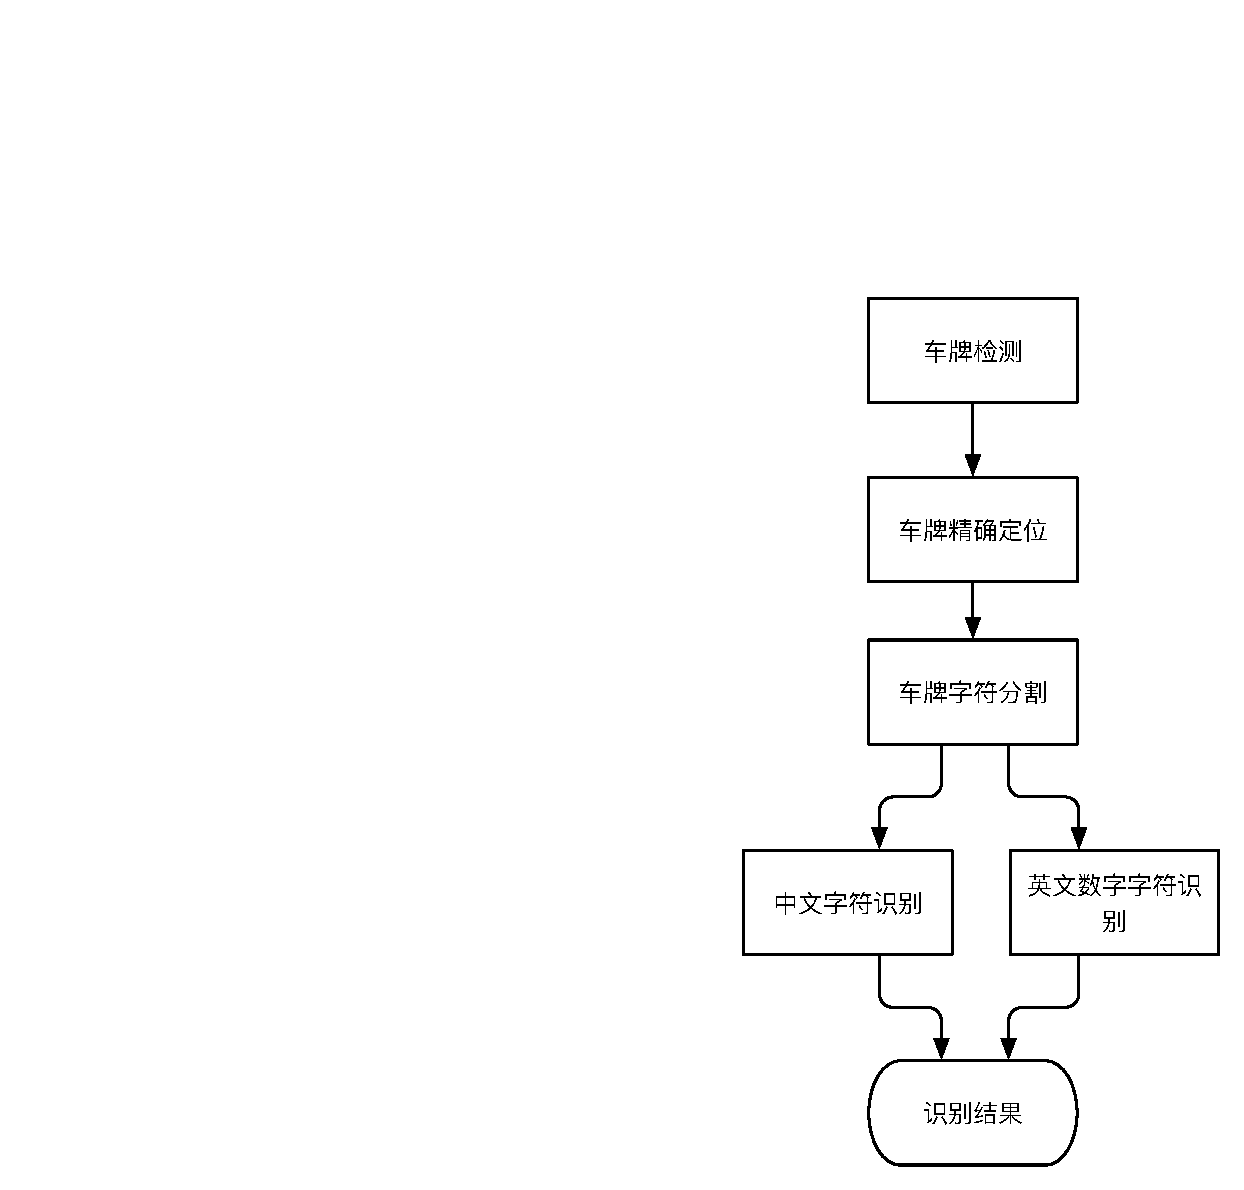
\includegraphics[height=0.5\textheight, keepaspectratio]{./Figure/SystemArch.eps}
  \caption{车牌识别系统结构图}\label{Fig:SystemArch}
\end{figure}

显然,车牌检测、车牌精确定位、车牌字符分割和车牌字符识别则是整个系统的核心和难点,
本文也着重对这四个子问题进行分析研究。

本文的内容安排如下:

第一章,为引言内容。介绍了课题研究的背景和意义。

第二章,为车牌精确定位方法研究。这一章首先介绍了CNN 的基本概念和原理,然后阐述如
何使用CNN 进行关键点回归以进行车牌的精确定位

第三章,为车牌的检测方法研究。这一章首先介绍了Region CNN(R-CNN)系列技术,包括
R-CNN、Fast R-CNN和Faster R-CNN。然后通过Faster R-CNN 技术实现了自然场景中车牌的检测。

第四章,为车牌字符分割方法方法研究。本章首先介绍了几种传统的车牌分割方法,并分析
了他们的优缺点。然后本章提出一种新的基于Extremal Region的方法进行车牌字符分割。

第五章,为车牌识别方法的研究。本章阐述如何通过卷积神经网络(CNN)技术进行车牌字
符识别,并进行相关实验。

第六章,为总结和展望。总结了本文的主要工作,并对未来的研究做了简单的介绍。

\section{本章小结}

本章从车牌识别的研究背景和研究意义展开讨论,说明了本研究的意义和价值;然后简要介
绍了两种研究思路——即传统方法和深度学习技术;最后简要说明了本文的内容安排。

\chapter{车牌精确定位}

在许多未使用深度学习技术的车牌识别系统中,倾向于使用边缘检测、Hough变换等寻找车
牌的边缘与顶点,直接实现车牌的检测与精确定位,但这些传统方法有着对图像质量、背景
颜色敏感,抗噪声能力差,难以处理特殊情况等诸多缺点,在很大程度上限制了其应用。因
此在本文中我们将车牌的定位分为车牌检测与车牌精确定位两步进行。其中车牌检测用于找
到图像中包含整个车牌的小区域,然后车牌精确定位则从这个小区域中找寻车牌的四个顶点
以进行精确定位。关于车牌检测技术将在本文第三章进行介绍,本章将介绍如何使用CNN 技
术进行车牌精确定位。在本章内容中,我们将车牌精确定位问题视为一个回归问题,然后讨
论如何使用CNN 对关键点进行回归的以实现精确定位,并进行实验验证。

\section{卷积神经网络概述}

卷积神经网络是一种前馈神经网络,有生物学家们在早期对猫视觉皮层的研究发展而来。
一个卷积神经网络一般由许多个卷积层和顶端的全连接层(对应经典的多
层感知机)组成,同时也包括相应的权重和池化层(Pooling Layer)。这一结构是的卷积
神经网络能够有效利用输入数据的二维结构,同时还极大程度减少了网络参数,降低了训练
难度和过拟合的风险。因此卷积神经网络在图像检测、识别方面取得了非常有优异的结构。
如2015年微软亚洲研究院Kaiming He等人发明的Residual Network成功的将ImageNet Top-5
错误率降低到了5\%左右\cite{He:2015tt}\cite{He:2016tq}。

\begin{figure}[ht]
  \centering
  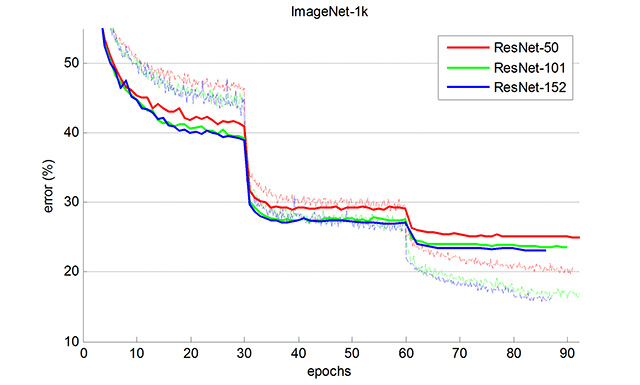
\includegraphics[width=0.8\linewidth]{./Figure/ResNetTrainError.jpg}
  \caption{文献\cite{He:2015tt}中Residual Network训练损失曲线}
\end{figure}

\subsection{卷积层}

所谓卷积层,是指使用一个相对较小的卷积核(Kernel)在整幅图像上滑动并进行卷积操作
并通过非线性激活函数从而得到输出的一种特殊的神经网络结构。常见的卷积核大小有 $1
\times 1, 3 \times 3, 5 \times 5, 7 \times 7$ 等。可以看到,卷积层通过权值共享和
稀疏连接两大特性,使之参数要远远少于具有相同输入输出大小的全连接层,参数的减少不
仅极大程度降低了网络的训练难度,而且有效避免了过拟合的出现。一般一个卷积层会有多
个卷积核,每一个卷积核可以提取图像的不同特征,从而得到不同的特征映射。图
\ref{Fig:LeNet} 是LeNet\cite{LeCun:1990vp}的网络结构,该网络由深度学习四巨头之
一的Yann LeCun 教授提出,并成功应用于手写数字识别问题\cite{LeCun:1990vp}。

\begin{figure}[ht]
  \centering
  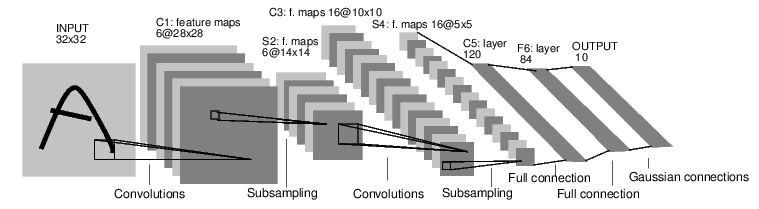
\includegraphics[width=0.8\linewidth]{./Figure/LeNet.png}
  \caption{用于手写数字识别的LeNet5\cite{LeCun:1990vp}} \label{Fig:LeNet}
\end{figure}

\subsection{池化层}

另一个关于卷积神经神经网络的重要概念是最大池化层,它是一种非线性降采样方法。

在实际应用中,经过卷积层所提取的特征映射仍可能维数较大,例如:对于一个 $32 \times
32$ 像素的图像,假设我们的卷积层包含512个卷积核,同时使用边缘填充技术(Padding)
使卷积输出与输入尺寸一样,则我们将一共得到 $512 \times 32 \times 32 = 524288$ 个
特征输出,这无论对于网络的储存、计算还是对训练数据集的需求都是十分巨大的,而且增
加了过拟合的风险。

因此我们在通过卷积层获取特征映射后,经常使用池化层对卷及特征进行将为。具体来讲,
我们卷积后得到的特征映射划分为 $n \times n$ 个子区域(子区域间可能重叠也可能不重
叠,取决于对池化层参数的定义),然后我们对每个子区域取其最大值(或平均值)所输出,
最后得到一个尺寸为 $n \times n$ 的特征映射,从而完成了对卷积特征映射的降维操作。

池化技术在计算机视觉中的应用价值有两个方面:

\begin{itemize}
\item 它减少了网络特征个数,从而降低了网络复杂度,使训练更容易进行而且不易出现过
  拟合
\item 这些池化单元使得CNN 具有了一定的平移不变性,即图像有小的位移时仍能保证提取
  的特征保持不变
\end{itemize}

\subsection{回归问题与$Smooth L_1$损失函数}

一般回归问题经常使用最小均方误差作为损失函数,但在许多回归问题上,人们倾向使
用$Smooth L_1$损失函数:

\begin{align}
smooth_{L_1}(x) = 
\begin{cases}
0.5x^2 & if |x| < 1 \\
|x| - 0.5 & otherwise \\
\end{cases}
\end{align}

\subsection{反向传播算法}

和其他机器学习算法一样,我们需要找到一种算法能够对神经网络进行训练。事实上,神经
网络的训练可以看作是一个最优化问题:

\begin{align}
\min_{\mathbf{w}}{Loss}
\end{align}

其中,$\mathbf{w}$神经网络模型参数,即每层神经元的权重,$Loss$代表损失值,用于度
量神经网络输出与真实值之间的误差大小。显然,这个优化问题是一个高维空间中的非凸优
化问题,不存在显式的解析解。一种常见做法是基于梯度的优化方法,即求取损失函数对参
数的梯度,并根据梯度对网络参数进行优化:

\begin{align}
\mathbf{w} = \mathbf{w} - \alpha\nabla_{\mathbf{w}}{Loss}
\end{align}

其中$\alpha$控制参数更新的程度,被称为学习率。于是现在我们的问题转换成了如何求取
损失关于网络参数的梯度$\nabla_{\mathbf{w}}{Loss}$。事实上,在多层感知机模型出现
之初,当时的神经网络研究者被这个问题困扰了10年之久,直到1986年前后Hinton 等人重新
发明反向传播算法,从而解决了这个问题。下面我们将简要介绍反向传播算法的原理。

为了叙述方便,我们定义如下记号:$\mathbf{a}^{l}$代表第l层网络的输出,
$\mathbf{w}^{l}$代表第l层网络的权重参数,$\sigma$代表激活函数,
$\mathbf{z}^{l}$满足$\mathbf{a}^{l} = \sigma(\mathbf{z}^{l})$,
$\mathbf{\delta}^{l} = \nabla_{\mathbf{z}^l}{Loss}$损失函数关于$\mathbf{z}^l$的
梯度。注意,上述粗体记号均为向量。根据上述定义和链式求导法则,我们可以得到以下方
程组:

\begin{align}
  \mathbf{\delta}^L = \nabla_{\mathbf{a}^L}{Loss} \odot \sigma'(\mathbf{z}^L) \\
  \mathbf{delta}^l = ((\mathbf{w}^{l+1}\mathbf{\delta}^{l+1})) \odot \sigma'(\mathbf{z}^l) \\
  \nabla_{\mathbf{w}^l}{Loss} = \mathbf{\delta}^l \times \mathbf{a}^{l-1} \\
\end{align}

其中,$\odot$表示向量汉密尔顿积,$\times$表示向量叉积(内积)。注意到在此方程组
中,损失函数关于$\mathbf{z}^l$的导数$\mathbf{\delta}$沿着网络反向传播,逐层向前
传递,即网络输出的误差在网络中逐层向前传递并据此修正网络参数$\mathbf{w}$,因此本
算法被称作\textit{反向传播}算法。

\section{Residual Network}

按照我们一般的经验,在不出现梯度耗散/梯度爆炸以及过拟合的情况下,CNN 应该是越深
效果越好。可是在实验中我们发现,当网络加深后,整个神经网络的错误率反而上升了,我
们称这种情况为Degradation。目前梯度耗散/梯度爆炸问题已经通过引入ReLU 激活函数而
被很好的解决\cite{Nair:2010vq},而随着大数据的出现过拟合问题也变得不是那么明显。
这时候限制神经网络走向更深的问题就只剩Degradation了。而微软亚洲研究院的Kaiming
He等人于2015年提出的Residual Network模型则很好的解决了Degradation问题,将网络层
数加深到了152层之多(最新的Residual Network已经达到1200层)。

Residual Network的思想是,既然我们使用梯度下降法使一个多层神经网络去逼近一个复杂
的非线性函数 $H(x)$ 会遇到Degradation问题而难以训练,那我们何不让这个多层网络去
逼近该映射测残差函数 $F(x) = H(x) - x$,我们猜想拟合残差函数会比拟合原函数容易一
些。虽然我们无法从数学上证明该结论,但是实验表明这种方法确实可行、有效。

图\ref{Fig:ResBlockActual} 所示的结构为构成被称之为Residual Block,其中的weight layer
一般是多个卷积层及配套的池化层。一个Residual Network由多个Residual Block堆叠而成。

\begin{figure}
  \centering
  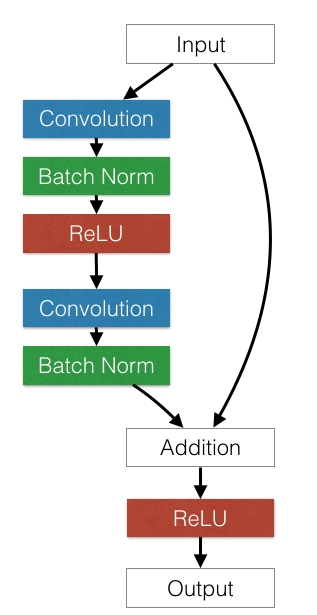
\includegraphics[height=0.5\textheight,
  keepaspectratio]{./Figure/ResBlockActual.png}
  \caption{用于ImageNet识别的Residual Network所使用的Residual
    Block}\label{Fig:ResBlockActual}
\end{figure}

\section{使用卷积神经网络进行车牌精确定位}

\subsection{数据处理}

在本文的实现中,我们首先将待处理的图片统一缩放至 $448 \times 224$ 的分辨率,并进
行零化和标准化操作,图像色彩空间选择为RGB 色彩空间。
此外,由于卷积神经网路不具有仿射不变性,因此我们需要对训练集进行数据扩张(Data
Augmentation),具体来讲就是对图片进行随机的旋转和放缩,从而增加CNN 抵抗仿射变换
的能力。

\subsection{模型设计}

车牌的精确定位问题可以看作一个对车牌四个顶点坐标进行回归的回归问题,因此我们可以
很容易的通过卷积神经网络搭建这样一个回归模型,其输入是经过缩放的车牌区域图片,输
出则是车牌四个顶点的坐标。本文并未从头训练一个全新的模型完成此任务,而是使用一个
训练好的模型,保留其卷积部分并将以Softmax 为激活函数的分类层更换为无激活函数的回
归层。具体来讲本文中使用的是训练好的34层Residual Network\cite{He:2015tt}模型,模
型结构如图 \ref{Fig:ResNet34Reg},其中前34个Residual Block为卷积特征提取,最后的
全连接层实现顶点坐标的回归。

\begin{figure}[ht]
  \centering
  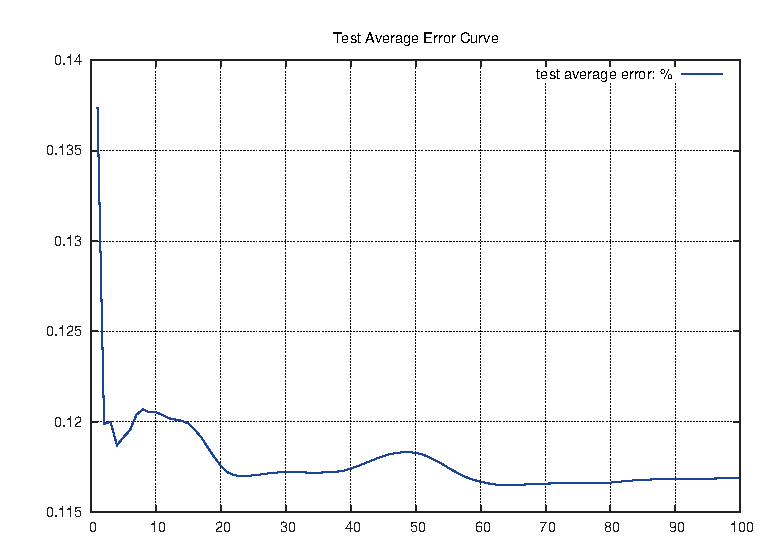
\includegraphics[width=0.8\linewidth]{./Figure/ResNet34Reg.eps}
  \caption{用于回归的34层Residual Network}\label{Fig:ResNet34Reg}
\end{figure}

\subsection{算法实现}

本章的神经网络模型使用Torch框架进行实现,实验机器配置见附录。

训练数据集大小为900张,测试数据集为100张,训练使用参数见表 \ref{Tab:LocationArgs}。

\begin{table}[ht]
\centering
\caption{车牌精确定位网络参数}\label{Tab:LocationArgs}
\begin{tabular}{|c|c|}
\hline
batch尺寸 & 25 \\
\hline
学习率 & 0.1 \\
\hline
GPU数量 & 2 \\
\hline
迭代次数 & 1000 \\
\hline
损失函数 & $Smooth L_1$损失函数 \\
\hline
优化算法 & Adam\cite{Kingma:2014us} \\
\hline
\end{tabular}
\end{table}

\subsection{实验结果与分析}

训练loss曲线
测试集上Mean Error和Max Error的曲线

结果图

可以看出,使用CNN 进行车牌精确定位可以较为有效的进行车牌定位,而且不需要手工选择
特征,鲁棒性强。但另一方面,由于神经网络的训练由于不需要先验知识,导致其对数据质
量和数量要求很高,而能否获取大量带标注的车牌数据进行训练,将直接影响这一步的结果。
相信如果能获得更大的带标注训练数据集,本算法的效果还有进一步提升的空间。

\section{本章小结}

本章主要简要介绍了CNN 的基本概念,然后基于34层的Residual Network设计了一个用于实现
车牌精确定位的卷积神经网络回归模型,并通过实验验证了其效果,证明了本方法的可行性。
最后提出通过增加训练数据集的大小,可以进一步提高模型的精度和效果。

\chapter{车牌检测}

所谓车牌检测,即是从一幅图像中找寻包含车牌的子图像,显然这属于目标检测(Object
Detection)问题。目标检测技术作为一个十分热门的研究领域,经历了从十年前HoG 方法大
行其道到如今R-CNN 技术一统天下的发展过程。R-CNN 技术于2014年由Ross Girshick等人提出,随后又出现
了Fast R-CNN和Faster R-CNN 两代的改进。如今, Faster R-CNN 技术不仅在Pascal VOC和
COCO 两个数据集上的目标检测任务中取得了最佳的效果,而且在借助GPU 加速的情况下做
到实时检测(0.2s/帧)。因此本章将首先简要介绍R-CNN 系列技术,然后在我们的数据集上
对其效果进行试验验证。

\section{R-CNN 概述}

\subsection{R-CNN}

传统的目标检测算法中,要对各种目标实现检测、定位和识别,一般分为三步:

\begin{itemize}
  \item 扫描图像产生可能的候选区域
  \item 对每个候选区域提取其特征
  \item 使用提取的特征对物体进行识别(背景也算为一类)
\end{itemize}

在R-CNN 技术(图 \ref{Fig:RCNN})中同样分为这三步,不同的是对每个proposal使用训练好的CNN 进行特征提取以
取代HoG 等传统手工特征。下面我们将分别对这三个步骤咋R-CNN 模型中的实现进行阐述。

\begin{figure}
  \centering
  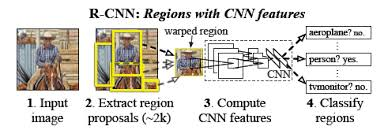
\includegraphics[width=0.8\linewidth]{./Figure/RCNN.jpg}
  \caption{R-CNN}\label{Fig:RCNN}
\end{figure}

\subsubsection{区域选择}

常用的候选区域选择算法有滑动窗口法、objectness、类别无关目标选择、Selective
Search等方法。出于对性能和效果的考虑,R-CNN 模型中选择使用 Selective Search进行目
标区域的选择。

\subsubsection{特征提取}

在R-CNN 模型中,我们使用一个在ImageNet 数据集上训练好的VGG 模型用作特征提取。我们摘
掉VGG模型最顶层的Softmax 分类层,将倒数第二层的4096维向量作为图像特征用于下一步的
目标识别。为了使每个候选区域符合VGG 网络的输入尺寸 ( $227 \times 227$像素RGB 图
像),我们将不同尺寸的目标候选区域统一缩放至$227 \times 227$像素进行处理。

\subsubsection{物体识别}

在模型的最后一步,我们使用SVM 对上一步得到的特征向量进行分类,以得到物体的类别。
注意到我们的类别包含 $N$ 个物体类和1个背景类一共 $N+1$ 类。

R-CNN模型使用CNN 提取特征的特性,使得它在Pascal VOC 数据集上的测试效果要好于所有传
统方法,成功将mAP (mean Average Precise) 提高到了53.7\%\cite{Girshick:2014jx},但
同时我们也注意到,模型中有两个重大缺陷:

\begin{itemize}
  \item 将不同尺寸的候选区域强制缩放至 $227 \times 227$ 会损失物体长宽比等许多信
    息
  \item 对每个候选区域分别使用VGG 网络提取特征使得整个识别过程速度十分缓慢,平
     均每幅图像需要40s之久\cite{Girshick:2014jx}。
\end{itemize}

\subsection{Fast R-CNN}

上一节末我们提到了原始的 R-CNN 模型有两大缺陷严重限制了其应用场景与范围。为了解决
这两大不足,Girshick在R-CNN 的基础上进行了改进,提出了 Fast R-CNN 模型
\cite{Girshick:2015ib},如图 \ref{Fig:FastRCNN}。相对于R-CNN,Fast R-CNN的改
进有两点:

\begin{itemize}
  \item 引入RoI 池化层
  \item 使用神经网络代替SVM 进行目标的检测与定位
\end{itemize}

\begin{figure}
  \centering
  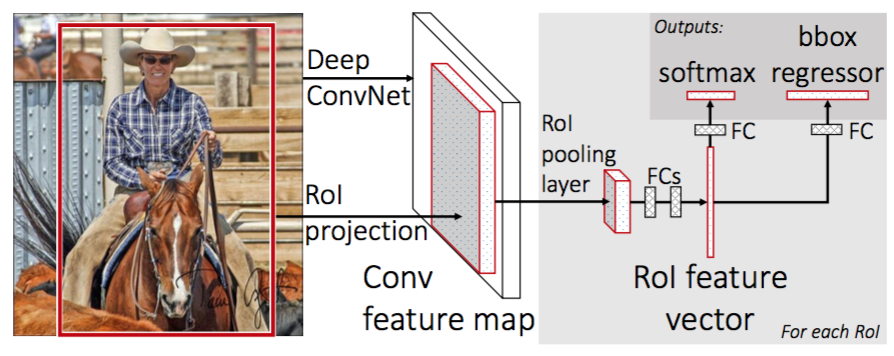
\includegraphics[width=0.8\linewidth]{./Figure/FastRCNN.png}
  \caption{Fast R-CNN\cite{Girshick:2015ib}}\label{Fig:FastRCNN}
\end{figure}

在原始的R-CNN 模型中,我们需要对每个候选区域进行尺寸缩放,并使用一个训练好的CNN 进
行特征提取,这一步使得 R-CNN 模型变得十分缓慢。因此我们自然的会考虑,我们是否可以
只对整幅图进行一次卷积,然后在提取到的卷积特征上直接提取每个候选区域的特征,避免
冗余的卷积计算和对候选区域尺寸的缩放。当然,答案是肯定的。

在Fast R-CNN 模型中,我们首先对整幅图像经过一系列卷积层和池化层产生一个卷积特征
映射。然后我们使用RoI 池化层从得到的特征映射图上提取每个候选区域的特征。

由于不同候选区域的尺寸是不同的,但是为了目标检测和识别,我们需要从特征映射上提取
出一个固定长度的向量作为区域特征,因此我们必须实现一种可以根据候选区域尺寸改变窗
口大小的特殊池化层,这种池化层被称为RoI 池化层。和普通池化层固定池化窗口的行为不
同,RoI 池化层的池化窗口大小随候选区域的大小而改变,而池化后的特征映射尺寸则固定。


具体来讲,我们定义一个 RoI 为一个四元组 $(r,c,h,w)$,其中 $(r,c)$ 为RoI 区域左上
角坐标,$(h, w)$ 为其长和宽。RoI 池化层将一个尺寸为 $h \times w$ 的RoI 区域分割成
$H \times W$ 个子窗口网格,每个窗口尺寸大约为 $\frac{h}{H} \times \frac{w}{W}$ ,
然后分别对每个网格窗口中的特征进行池化操作,最后得到的尺寸为 $H \times W$ 的特征
映射为RoI 池化层的输出。同时注意到RoI 池化层在反向传播时,梯度公式与普通池化层是
不同的,RoI 池化层的反向传播公式如下:

\begin{align}
\frac{\partial L}{\partial x_i} = \sum_{i}\sum_{j}[i = i^*(r,j)]\frac{\partial
  L}{\partial y_{rj}}
\end{align}

其中$y_{rj} = x_{i^*(r,j)}$,$i^*(r,j) = \arg\max_{i'\inR(r,j)}x_{i'}$,$R(r,j)$
为产生输出单元$y_{rj}$的池化窗口中包含的元素坐标集合。

在通过RoI 层为每个候选区域提取了 $H \times W$ 维特征后,这些特征被送入一个多层感知
机中,与R-CNN 中使用SVM 进行物体识别不同,这个多层感知机有两个输出:

\begin{itemize}
  \item 目标的类别
  \item 目标的边界矩形bbox(bounding box)
\end{itemize}

由于使用了神经神经网路代替了SVM进行分类和bbox 回归,使得整个Fast R-CNN可以作为一
个完整的神经网络在GPU 中执行,从而避免了显存和主存间的数据复制,极大程度提高了计
算性能。

由于整个网络有两个输出:目标的类别和bbox,因此整个网络的损失函数不能再是简单的交
叉熵损失或者最小二乘损失。在此,作者针对Fast R-CNN 提出了一种特殊的多任务损失函
数。我们定义第一个输出为目标在$K+1$个类别(背景也算一类)上的概率分布 $p = (p_0,
\cdots, p_K)$ ,第二层的输出为目标的bbox 坐标尺寸 —— $t_k = (t_x^k, t_y^k, t_w^k, t_h^k)$,其
中$k$代表该bbox 为第$k$个物体类别。此外,对每个用于训练的RoI,我们定义真实类别为
$u$,真实bbox 坐标为$v$。我们定义每个RoI 的多任务损失函数$L$如下:

\begin{align}
L(p, u, t^u, v) = L_{cls}(p, u) + \lambda[u \geq 1]L_{loc}(t^u, v)
\end{align}

其中,$[u \geq 1]$为指示函数——当$u$大于等于1时为1,否则为0。目标分类的损失函数
$L_{cls}(p,u) = -\log{p_u}$为对真实类别$u$的对数损失函数。bbox 回归任务的损失函数
$L_{loc}(t^u,v)$定义如下:

\begin{align}
L_{loc}(t^u, v) = \sum_{i\in \{x,y,w,h\}}{smooth_{L_1}(t_i^u-v_i)}
\end{align}

在有些时候我们也会用最小二乘损失代替$Smooth_{L_1}$损失函数。

有了如上的结构定义,我们就可以通过梯度下降法对整个Fast R-CNN进行训练。文献
\cite{Girshick:2015ib}中的实验结果表明,Fast R-CNN在Pascal VOC数据集上mAP可以达
到70.0\%,一举超越R-CNN和SPPnet 而夺得头筹。但是另一方面,虽然Fast R-CNN的速度较
R-CNN有了很大的提升,但仍旧未能达到实时级别,还需进一步改进。

\subsection{Faster R-CNN}

虽然Fast R-CNN 算法在目标识别问题上已能达到准实时的速度,然而这阻挡不了科学家追求
更快、更好的脚步。因此微软亚洲研究院的Shaoqing Ren等人在Fast R-CNN 的基础上提出了
速度更快的Faster R-CNN算法\cite{Ren:2015ug}(值得一提的是,也正是该组于2015年提出了Residual
Network,笔者对他们的科研实力只能佩服不已)。分析发现,使用Selective Search的方
法进行目标候选区域选择是制约Fast R-CNN 性能的瓶颈,因此一个很自然的想法便是能否
使用基于神经网络的方法进行候选区域的选择以替代速度缓慢的Selective Search方法。
Ren 等人正是基于这一思想,创造性的提出Region Proposal Network (RPN),将R-CNN 的整个
流程归纳进神经网络框架内,进一步提高了检测速度,在GPU 加速的帮助下达到了实时级别
的性能(图 \ref{Fig:FasterRCNN})。

\begin{figure}[ht]
  \centering
  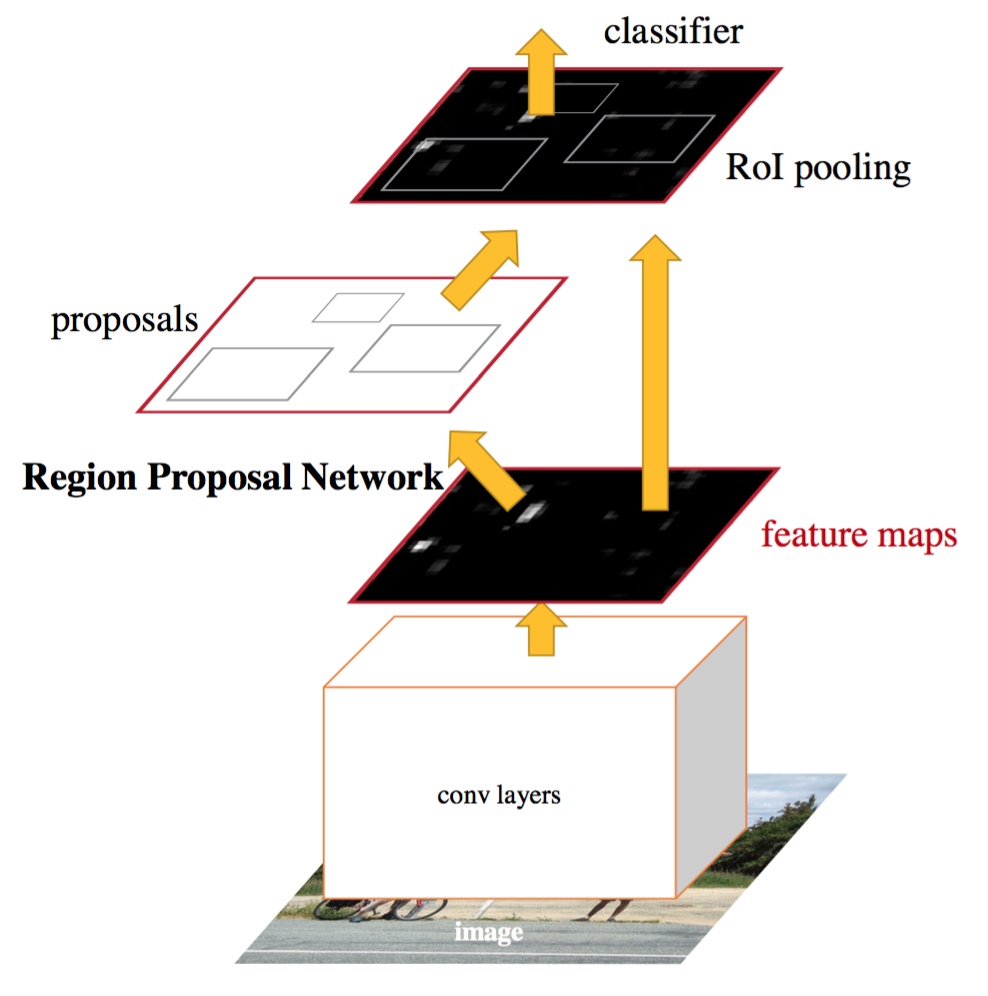
\includegraphics[width=0.8\linewidth]{./Figure/FasterRCNN.png}
  \caption{Faster R-CNN\cite{Ren:2015ug}}\label{Fig:FasterRCNN}
\end{figure}

RPN网络以Fast R-CNN 网络中经由卷积层提取的卷积特征映射作为输入,并以此产生一系列
矩形候选区域,并对每个区域为一个目标的可能性打分。为了生成候选区域,RPN 使用一个
小型卷积神经网路在特征映射图上滑动,这个小型网络输入为特征映射图上一个尺寸为$n
\times n$窗口,然后该窗口内的特征将通过RoI 池化的方式被映射为一个256维的向量(有
时也用512维,取决于计算特征映射所用卷积网络的复杂度)。最后,这256维特征将被送入两个独
立的全连接层中——一个全连接层用于目标分类(记为\textit{分类层}),另一个用于目标
位置回归(记为\textit{回归层})。整个RPN 结构如图 \ref{Fig:RPN} 所示。

\begin{figure}[ht]
  \centering
  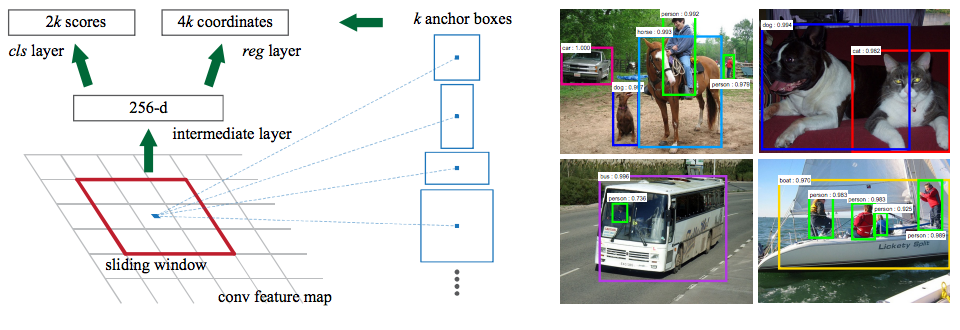
\includegraphics[width=0.8\linewidth]{./Figure/RPN.png}
  \caption{Region Proposal Network\cite{Ren:2015ug}}\label{Fig:RPN}
\end{figure}

但是光有上述固定的网络无法处理不同尺寸、不同长宽比的目标物体,为了使RPN 能够处理
不同尺寸、长宽比的物体,作者提出了Anchor的概念。我们在滑动窗口每次滑到的位置,
我们一共提出$k$个尺寸、长宽比不同的候选区域,每一个这样的区域成为一个Anchor。所
以我们网络的\textit{分类层}有$2k$个输出,为每个Anchor是目标物体/背景的概率,网络
的\textit{回归层}有$4k$个出书,为每个Anchor的坐标。一般在一个位置,我们使用3个不
同尺寸放缩比和3个不同长宽比共生成9个Anchor。对一个尺寸为$W \times H$的特征映射图,
我们共产生$WHk$个Anchor。

为了训练RPN,我们需要为每一个Anchor提供一个二元标签(代表是物体还是是背景)。我
们将两类Anchor标记为正例(是物体):(1) 该Anchor和真实的边框有最高的
Intersection-over-Union(IoU) 重叠,或者(2) 该Anchor和任一个真实的边框的IoU重叠都
高于0.7。值得注意的是,根据这种标记方法,一个真实的边框可能会产生多个标记为正例
的Anchor。有了如上对标记的定义,我们的损失函数定义如下:

\begin{align}
L(\{p_i\}, \{t_i\}) = \frac{1}{N_{cls}}\sum_i{L_{cls}(p_i, p_i^*)} + \lambda\frac{1}{N_{reg}}\sum_i{p_i^*L_{reg}(t_i,t_i^*)}
\end{align}

在此,$i$为Anchor的下标,$p_i$代表第$i$个Anchor是一个目标物体的概率,$p_i^*$为真
实值,当Anchor为正例是$p_i^* = 1$,否则是0 。$t_i$是一个四元组,包含表示Anchor坐
边框坐标的四个值,$t_i^*$则是相应的真实值。此外,$L_{cls}$是常用语二分类问题的对
数损失函数,$L_{reg}$则同Fast R-CNN 一样使用$Smooth L_1/$损失函数。此外,
$N_{cls}$和$N_{reg}$为两个归一化参数,在实现中常取$N_{cls}$为mini-batch的大小,
而$N_{reg}$取不同位置Anchor的数量。此外,由于RPN 在很多时候生成的候选区域彼此有
很大的重叠,因此我们基于RPN 网络对区域为目标物体可能性的打分,使用非极大抑制
(NMS)对候选区域进行筛选,从而减少计算量。

综上所述,可以看出来Faster R-CNN实际上是由RPN和Fast R-CNN 组合而成,因此我们在训
练Faster RCNN 时需要分别训练这两个网络。但是这两个网络并非完全独立,而是有着共享
的卷积部分,因此如何才能正确的训练整个网络也是一个需要解决的问题。在Faster R-CNN
的文献\cite{Ren:2015ug}中,作者提出了一种4步训练法:第一步,我们使用预训练好的模型
初始化RPN 的卷积部分,并单独训练RPN 网络,包括共用的卷积部分。第二步,我们使用预
训练好的模型初始化Fast R-CNN 的卷积部分,并使用上一步训练好的RPN 网络产生候选区
域来训练Fast R-CNN 的识别网络。到这一步为止,RPN和Fast R-CNN 并不共享彼此的卷积部
分。第三步,我们使用Fast R-CNN的卷积部分初始化RPN 的卷积部分,这时候两个网络共享
同样的卷积层,此时我们固定卷积层,对RPN 独有的分类层和回归层进行训练。最后一步,
我们仍旧固定卷卷积部分,对Fast R-CNN 的分类、回归层进行训练。最后我们得到的两个
网络共享同样的卷积层,但是却是不同的网络。

Faster R-CNN技术不仅在Pascal VOC数据集和COCO数据集上取得了和Fast R-CNN 比肩的出色
效果,而且在GPU 加速的帮助下可以达到17fps 的处理速度,基本满足对实时性的需求。
Faster R-CNN 无疑已成为时下最主流的物体识别技术之一。

\section{使用Faster R-CNN 进行车牌检测}

由于Faster R-CNN 在物体识别领域有着速度快、准确率高、鲁棒性好、人工干预少等优点,
我们自然可以联想到将此技术用于车牌检测工作。下面我们将介绍如何使用Faster R-CNN实
现车牌检测。

\subsection{数据集准备}

\subsubsection{车牌图片}
本文选择了1000张在道路上拍摄的含有车牌的照片,注意这些照片为步行或行车过程中使用
手机拍摄而来,存在大量倾斜、变形的情况。

\subsubsection{数据标注}
本文中首先对这些车牌的四个顶点进行手工标注,然后取包含车牌区域的最小外接矩形作为
bbox用于Faster R-CNN 的训练。 

\subsection{实现环境}

本文的Faster R-CNN 实现基于开源项目 py-faster-rcnn
\footnote{https://github.com/rbgirshick/py-faster-rcnn.git}修改而来,增加了对上
一步构造出的车牌数据的支持。

训练网络使用的工作站配置见附录中表 \ref{Tab:WorkstationInfo}。

训练数据集图片为900张,测试数据集图片为100张,模型参数见表 \ref{Tab:FasterRCNNArgs}。

\begin{table}[ht]
\centering
\caption{Faster R-CNN参数}\label{Tab:FasterRCNNArgs}
\begin{tabular}{|c|c|}
\hline
训练第一步迭代次数 & 80000 \\
\hline
训练第二步迭代次数 & 40000 \\
\hline 
训练第三步迭代次数 & 80000 \\
\hline 
训练第四步迭代次数 & 40000 \\
\hline
\end{tabular}
\end{table}

\subsection{实验结果与分析}

经过训练,Faster R-CNN在100张测试数据集上精度达到84.54\%,相信如果换用更大的训练
数据集后效果还可进一步提升。

\begin{figure}[ht]
\centering
\subcaptionbox{分类损失曲线}
{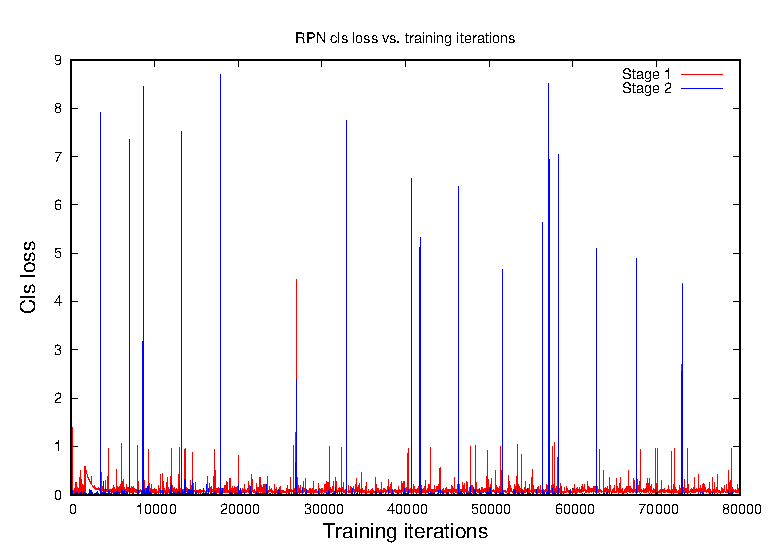
\includegraphics[width=0.8\linewidth]{./Figure/RPNClsLoss.eps}}
\subcaptionbox{BBox 回归损失曲线}
{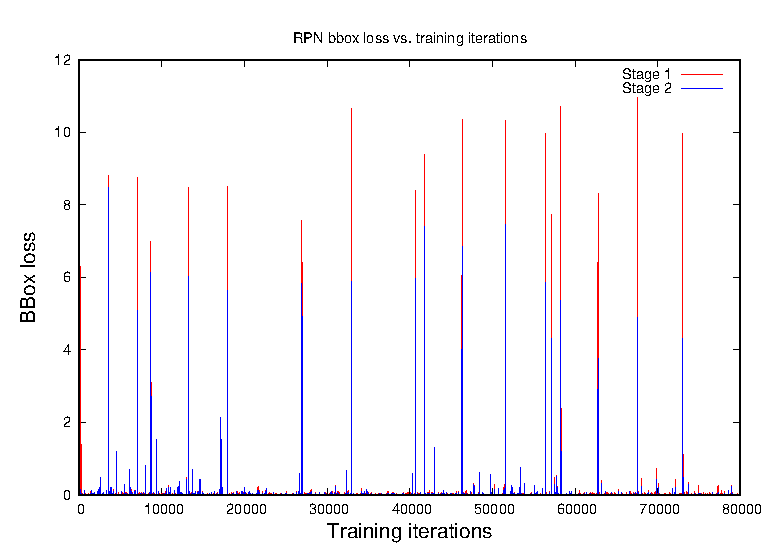
\includegraphics[width=0.8\linewidth]{./Figure/RPNBBoxLoss.eps}}
\caption{RPN训练损失曲线}
\end{figure}

\begin{figure}[ht]
\centering
\subcaptionbox{分类损失曲线}
{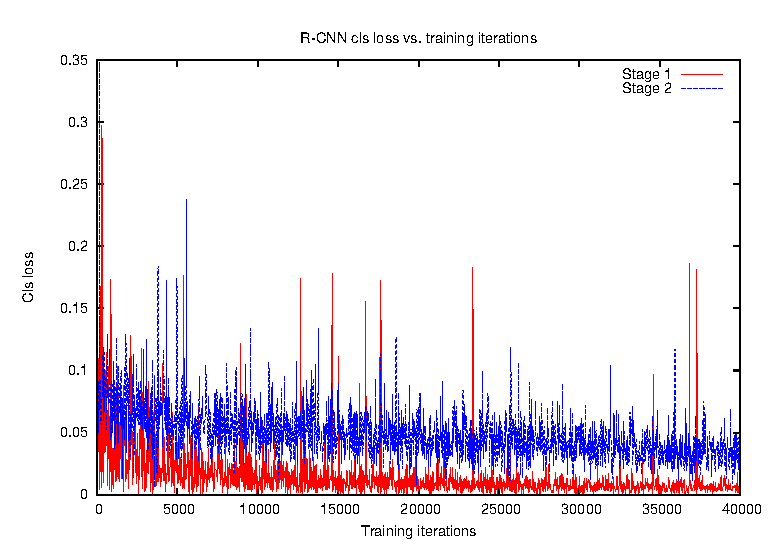
\includegraphics[width=0.8\linewidth]{./Figure/RCNNClsLoss.eps}}
\subcaptionbox{BBox 回归损失曲线}
{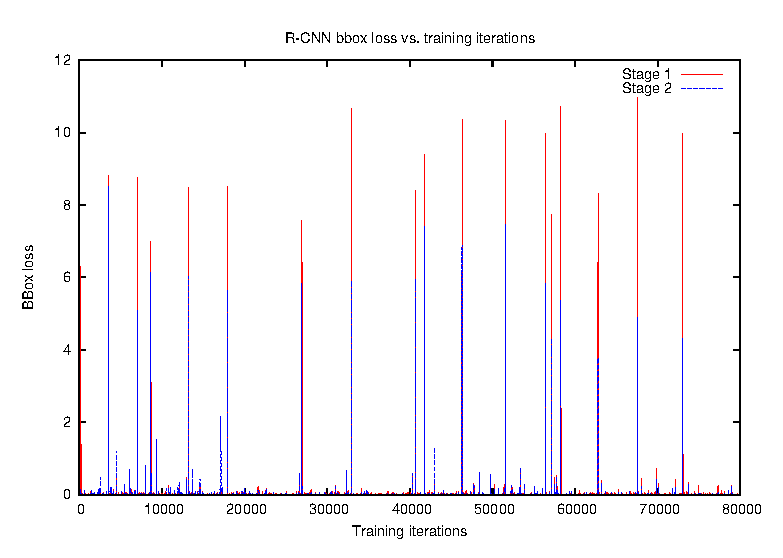
\includegraphics[width=0.8\linewidth]{./Figure/RCNNBBoxLoss.eps}}
\caption{Fast R-CNN训练损失曲线}
\end{figure}

\section{本章小结}

本章首先介绍了使用R-CNN 系列算法进行物体检测的基本原理,然后通过修改开源项目
py-faster-rcnn,在我们的车牌数据集上进行训练,最后验证其mAP 可以达到85\%左
右,验证了使用Faster R-CNN 进行车牌检测的有效性。

\chapter{车牌字符分割}

传统的车牌字符分割有两种方法——基于连通域的分割方法和基于直方图垂直投影的分割方法。
但这两种方法非常显著的缺点:一方面,基于连通域的方法取决于对车牌进行二值化操作的效
果,而由于车牌受光照、拍摄角度、天气、污损等因素的影响,很难找到一种完美的二值化
操作方法对图像进行二值化,这大大影响了连通域方法的效果;另一方面,基于直方图垂直
投影的方法只能处理绝对水平的车牌,对存在倾斜、错切变形的车牌则无能为力,甚至相机
抖动所产生的图像模糊也会影响该方法的效果,使之无法准确分割。因此本文放弃传统上述
两种思路,尝试从字符检测与提取的角度来处理车牌字符分割问题。

\section{Extremal Region综述}

\subsection{Extremal Region}

我们首先定义一幅图像$\mathbf{I}$为一个映射$\mathbf{I} : \mathcal{D} \subset
\mathbb{N}^2 \rightarrow \mathcal{V}$,其中$\mathcal{V}$一般为
$\{0,\cdots,255\}^3$(即一个色彩空间)。然后,我们定义图像的一个通道为
$\mathbf{C} : \mathcal{D} \rightarrow \mathcal{S}$,其中$\mathcal{S}$为一个全序
集并且存在一个映射$f_c : \mathcal{V} \rightarrow \mathbf{S}$将像素值映射到该全序
集。我们定义$A$为邻接关系$A \subset \mathcal{D} \times \mathcal{D}$,常见的邻接
关系有4-邻接和8-邻接,在本章的实现中我们使用4-邻接关系。

我们定义图像$I$(或通道$C$)的一个Region为$\mathcal{D}$的一个连续子集(所为连续,
是指$\forall{p_i, p_j \in \mathcal{R}}, \exists{p_i, q_1, q_2, \cdots, q_n,
  p_j} : p_iAq_1, q_1Aq_2,\cdots,q_nAp_j$。我们定义Region边界
$\partial{\mathcal{R}}$为那些与Region$\mathcal{R}$邻接却不属于$\mathcal{R}$的像
素的集合,即$\partial{\mathcal{R}} = \{p \in \mathcal{D} \\ \mathcal{R} :
\exists{q \in \mathcal{R}} : pAq \}$。现在,我们定义\textit{Extremal Region}(ER)
为那些边界像素值比内部像素高许多的Region,写成数学语言即$\forall{p \in
  \mathcal{R}}, q \in \partial{\mathcal{R}} : \mathbf{C}(q) > \theta > \mathbf{C}(p)$,其中
$\theta$为ER 的阈值。由上式的定义,我们注意到一个阈值为$\theta$的ER $r$可以由多个或
零个阈值为$\theta - 1$的ER 和值为$\theta$的像素和并集:$r = \left( \bigcup{u \in
    R_{\theta-1}} \right) \cup \left( \bigcup{p \ in \mathcal{D} : \mathbf{C}(p)
  = \theta} \right)$构成,,其中\(R_{\theta-1}\)表示阈值为\(\theta_1\)的 ER。这
一性质将用于下一节计算CSER 的过程中。

\subsection{Class-specific Extremal Region}

由上一节可知,对于一幅图像,字符区域一定是ER,但反之不然。因此,对于字符提取任务,
我们只需要将一幅图像的ER 中非字符的那些去掉,只保留字符区域的ER 即可,这样,我们
的问题就转换为如何识别一个ER 是否包含有效的字符这一判定问题。而Class-specific
Extremal Region(CSER)\cite{Neumann:2012ik}的核心思想正是通过机器学习的方法,使用一个分类器对ER进行筛
选,从而快速准确地提取图像中的字符区域。因此整个CSER 算法可以归结为两部分:ER区域
的产生和ER 区域的判别。

\subsubsection{ER的搜索}

由于阈值为$\theta$的ER 可以由阈值为$\theta-1$的ER 区域所产生,因此我们可以从0开
始逐步增加阈值$\theta$从而逐步产生ER,这些ER 根据其产生关系可以组成一个树状结构
(如图\ref{Fig:ERTree},我们对ER 的搜索过程便是自顶向下遍历这棵树的过程。但是,
这棵树往往包含数量巨大的ER 区域,若不对搜索过程进行剪枝,则无论是在时间上还是内
存上都将难以承受。因此,我们在搜索过程中对每个ER 使用识别器进行判别,若其为字符
区域的概率小于给定阈值,我们则放弃在该节点上的进一步搜索(即剪枝),从而减少大量
不必要的计算。下一节,我们将描述如何设计这种分类器,以实现对ER 的判别。

\begin{figure}[ht]
  \centering
  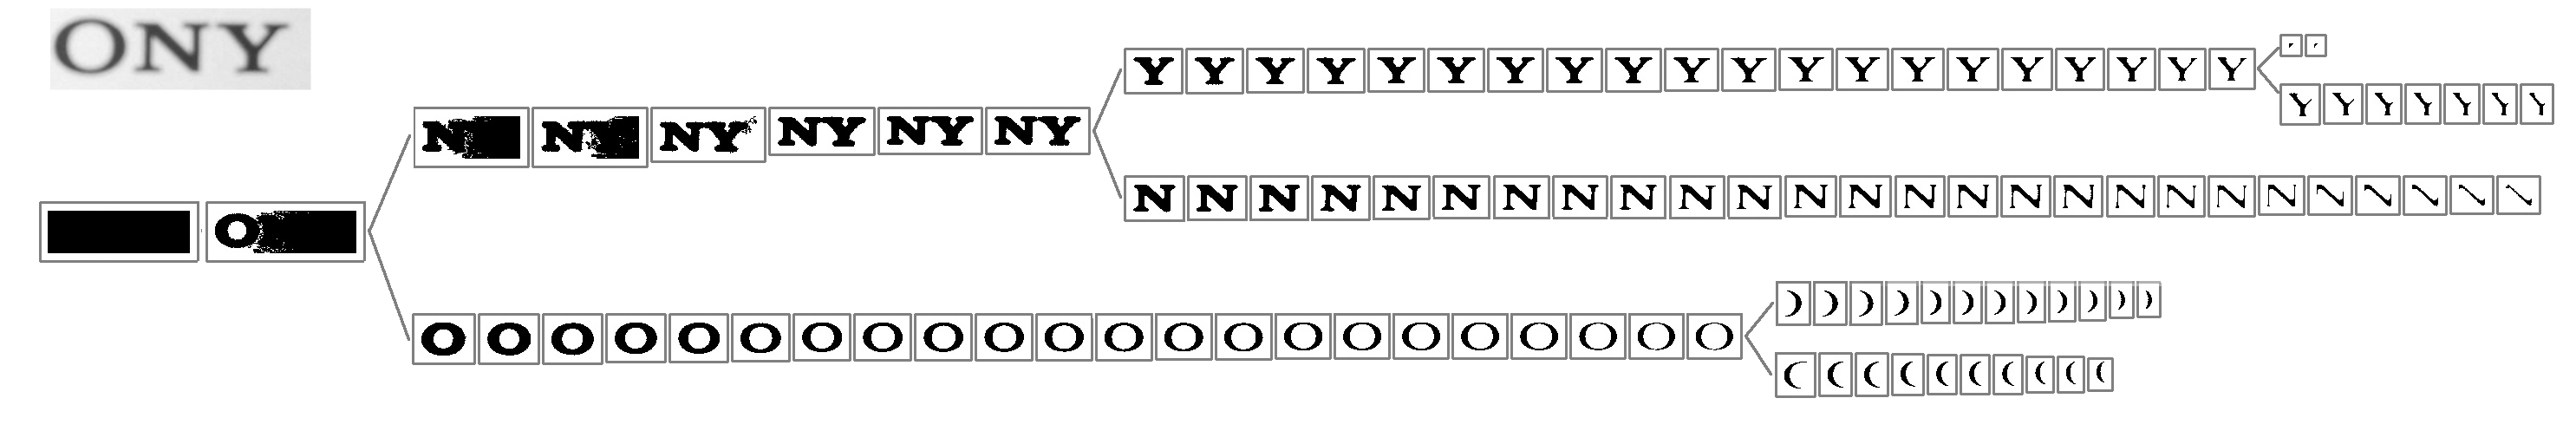
\includegraphics[width=0.8\linewidth]{./Figure/ERTree.png}
  \caption{ER搜索过程中产生的搜索树}\label{Fig:ERTree}
\end{figure}

\subsubsection{ER的判别}

若要实现对ER 区域的判别,最简单也是最理想的情况是使用一个复杂分类器(如SVM、CNN)
直接对ER 区域的图像进行判别。但是此种分类器往往相对较慢,无法达到对实时性的要求。
因此Neumann等人在发明CSER 时提出使用一些能够快速计算且效果良好的简单特征作为分类
器的输入进行分类。注意到,我们使用CSER进行字符ER 提取的时候一共使用了两次分类器——第
一次是使用分类器对ER 搜索树进行剪枝,第二次则为最终输出时对ER 区域进行判别和筛选。
显然,这两次对分类器的使用有着不同的要求:用于搜索的分类器对精度要求低但要求计算
速度快;而用于最终输出的分类器对性能要求不高但要求精度更高。因此,我们在此分别设
计这两个分类器,对于搜索过程中使用的分类器(下文中将称之为分类器1)我们使用少但
容易计算的特征进行分类,而对于最终输出时使用的分类器(下文中将称之为分类器2)我们使用计
算量更大但更有效的特征进行分类。

为了性能需要,我们希望对于阈值为$\theta$的ER 的特征可以从
$\theta-1$的ER 是的特征快速计算得出,即假设我们已知特征 $\phi(u), \forall{u \in
  R_{\theta-1}}$,我们希望对每个阈值为$\theta$的ER $r = \left(
  \bigcup{u \in R_{\theta-1}} \right) \cup \left( \bigcup{p \in \mathcal{D}} :
  \mathbf{C}(p) = \theta \right)$,其特征$\phi(r) = \left( \oplus{\phi(u)}
\right) \oplus \left( \oplus{\psi(p)} \right)$,其中$\psi(p)$被称为初始化函数,
$\oplus$代表将特征进行合并的算子。作者称这类特征可增量计算描述子。在文献
\cite{Neumann:2012ik}中,作者首先定义了如下可增量计算描述子:

\begin{itemize}
\item \textbf{面积$a$}:ER 区域的面积(即像素数量)。
\item \textbf{边框($x_{min}, y_{min}, x_{max}, y_{max}$}:ER区域的右上角和左下角坐标。
\item \textbf{周长$p$}:ER 区域边界的长度(即像素数量)。
\item \textbf{欧拉数$\eta$}:欧拉数是二值图像的一种拓扑特征,为连通域数目和孔洞
  数目之差。
\item \textbf{水平交叉点数$c_i$}:用一个长度为图像高度的向量来保存对应行像素在属于ER与不属于ER 之间转变的次数。
\end{itemize}

对于以上描述子,我们可以很容易的找到其对应的初始化函数$\psi(p)$和合并算子
$\oplus$。

对于分类器1,我们基于基于上面的描述子使用如下特征:

\begin{itemize}
\item \textbf{长宽比}($w/h$)
\item \textbf{compactness}($\sqrt{a}/p$)
\item \textbf{孔洞数}($1-\eta$)
\item \textbf{水平交叉点特征}($\hat{c}=median(\mathbf{c}_{\frac{1}{6}w}, \mathbf{c}_{\frac{3}{6}w}, \mathbf{c}_{\frac{5}{6}w})$)
\end{itemize}

对于分类器2,由于我们需要其精度更高,因此我们额外使用如下特征:

\begin{itemize}
\item \textbf{孔洞面积比$a_h/a$}:其中$a_h$代表ER 区域内孔洞的面积(像素数)。
\item \textbf{凸包面积比$a_c/a$}:其中$a_c$为ER 区域凸包的面积。
\item \textbf{外轮廓拐点数$\kappa$}:代表ER 区域边界凹角与凸角的变化数目。
\end{itemize}

此外,为了平衡性能与训练难度,两个分类器我们均采用基于决策树的AdaBoost分类器。

\section{使用Class-specific Extremal Region进行车牌字符分割}

\subsection{算法设计}

\subsubsection{候选区域的提取}

我们首先将一幅图像划分为$R,G,B,-R,-G,-B,\nabla$七个通道,其中$R,G,B$为红、绿、蓝
三色通道,$-R,-G,-B$为对相应颜色通道进行反转所得到的通道,$\nabla$为梯度。然后我
们分别对这些通道提取CSER作为候选区域。

\subsubsection{候选区域的进一步筛选}

得到所有CSER 后,仍不免有很多误判和包含不完整字符的区域(如图\ref{Fig:AllERs}),
在此我们就需要使用一些车牌字符的性质对这些候选区域进行进一步筛选。

\begin{figure}[ht]
  \centering
  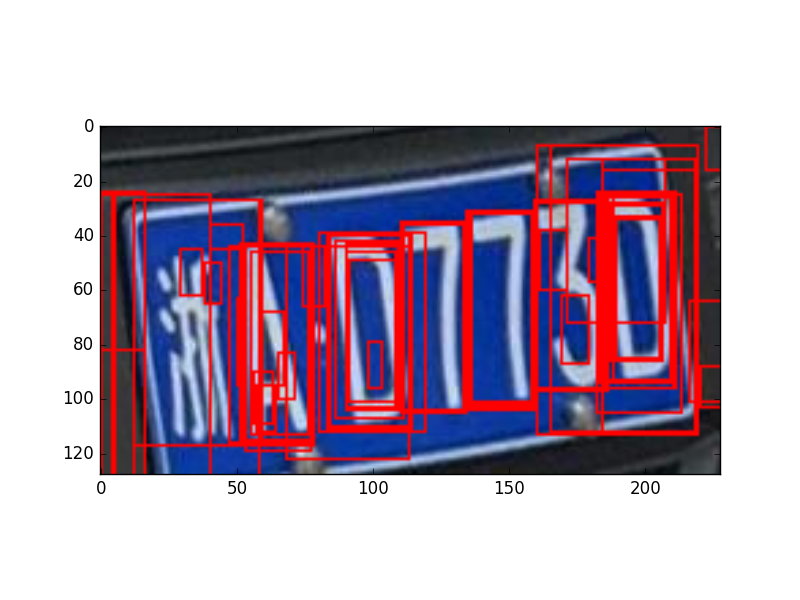
\includegraphics[width=0.8\linewidth]{./Figure/AllERs.png}
  \caption{使用CSER提取出的所有候选区}\label{Fig:AllERs}
\end{figure}

在我们的算法中我们从如下方面对候选字符区域进行筛选:

\begin{itemize}
\item \textbf{长宽比} 根据中华人民共和国公共安全行业标准GA36— 2007中关于车牌的相关
  规定,我们限定候选字符的长宽比在区间0.3到10之间
\item \textbf{尺寸} 我们根据候选区域相对于图像的尺寸,去除那些过大或过小的区域
\item \textbf{区域中心位置} 根据区域的中心位置,合并那些IoU 较大的候选区域,去除
  不可行的区域
\end{itemize} 

此外,有时候可能会出现缺失部分字符的情况,在这种时候我们将根据已取得的字符位置和
尺寸,对缺失的字符区域进行推算。

通过上述步骤,最终我们得到车牌中后六个字符的位置(即英文和数字部分),接下来,我
们将通过这六个字符的位置推算中文字符位置

\subsubsection{中文字符的处理}

由于CSER 是基于连通域进行字符提取的,因此它无法直接处理中文这种由多个连通域组成
的字符(如“穿”、“京”)。为了解决这一问题,在本文中我们使用的方法是,仅使用CSER
提取车牌中的英文和数字,然后根据车牌的结构特点和字符间的相对位置关系对中文字符的
位置进行推算。

\subsection{算法实现}

CSER的相关算法已经在最新版的OpenCV
Contrib\footnote{https://github.com/Itseez/opencv\_contrib}中得以实现;CSER所使用
的两个分类器的训练则由作者基于OpenCV使用C++开发完成;最后整个字符分割模块使用
Python语言和最新版的OpenCV(需手工编译最新版)开发完成。

\subsection{实验效果}

\begin{figure}[th]
\centering
\subcaptionbox{示例1}
{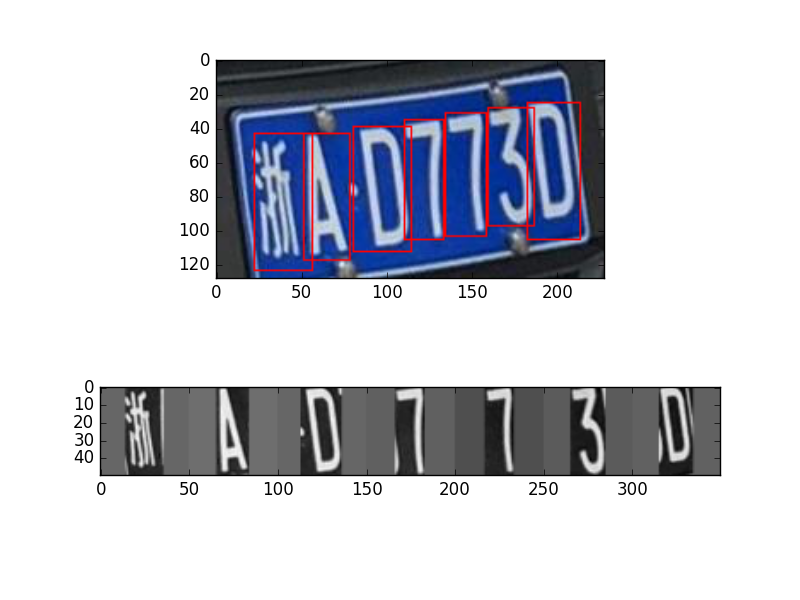
\includegraphics[width=1\linewidth]{./Figure/TextSegmentation.png}}
\subcaptionbox{示例1}
{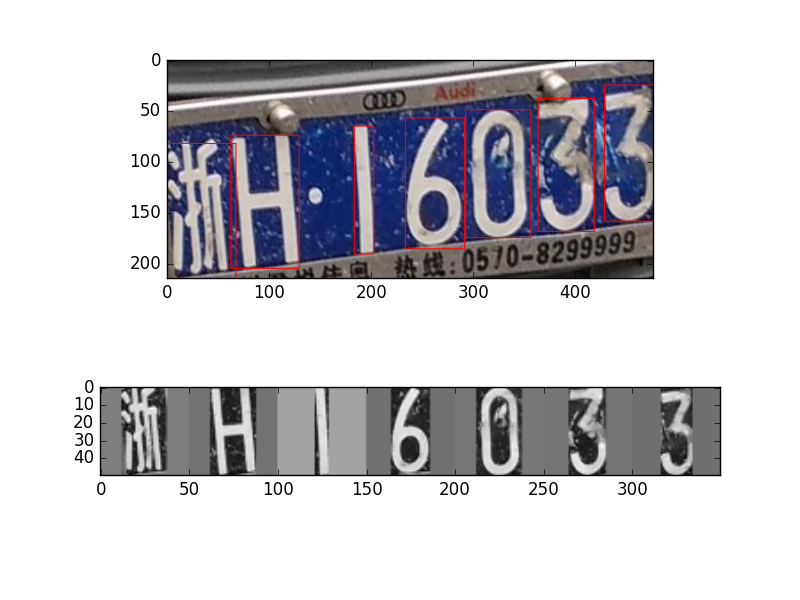
\includegraphics[width=1\linewidth]{./Figure/TextSegmentation2.png}}
\caption{车牌字符分割}\label{Fig:TextSeg}
\end{figure}

可以看出基于CSER 的车牌分割方法即使在车牌有旋转、变形、污损的情况下,仍可以准确
的从车牌图像中找寻到字符外接轮廓,具有极强的鲁棒性,且检测速度快,非常适用于车牌
识别系统中并代替传统的字符分割方法。

\subsection{本章小结}

本章受自然场景中字符识别任务的启发,提出使用CSER 技术对车牌图像中的字符进行分割、
提取,克服了传统方法的诸多缺点,具有准确率高、鲁棒性强、性能好等特点。但是另一方
面,本方法仍称不上完美,还有许多可以改进的空间:其一,CSER 对字符区域的提取基于连
通域,而中文字符由于其往往包含多个连通域(如“川”字),因此不能直接使用CSER 技术进
行提取,一种可行的改进是使用\cite{Neumann:2011dy}中提出的搜索方法对ER 区域进行合
并操作,以求取中文字符;另一方面,可以在CSER 算法中加入非极大抑制来对ER 进行预筛
选。此外,由于CSER 算法具有并行的特点,因此可以考虑进行GPU 加速来提升执行性能。

\chapter{车牌字符识别}

车牌识别是车牌识别系统最后也是最关键的一步,幸运的是,字符识别问题已经被人们充分
的研究了几十年,并且提出了一系列十分有效的方法。早期的字符识别系统中经常使用SVM 
作为分类器对字符进行识别,但是随着深度学习的发展,人们发现CNN 能在字符识别任务上
取得非常优秀的效果,因此越来越的字符识别系统选择使用CNN 作为其字符识别算法。本文
也采用了CNN 对车牌字符进行识别,下面对此进行描述。

\section{使用CNN 进行多类别分类}

在前几章中我们已多次使用CNN 来完成回归任务,并使用$Smooth L_1$损失函数进行梯度下
降优化。虽然,分类任务可以看做是一种特殊的回归任务,但显然是$Smooth L_1$损失函数
并不适合于分类问题。下面我们将介绍用于回归问题的Softmax 激活函数和交叉熵损失函数。

\subsection{Softmax激活函数}

对于分类任务,首先我们考虑如何表示类别信息,目前最常用的表示方法当属One-Hot表示
法——即对于一个$N$类别分类问题,我们使用一个N元组 $(p_1, \cdots, p_N)$ 表示其类别信
息,其中$p_i$为目标属于第$i$类的概率。例如,对于真实类别为$j$的目标,可令$p_j$等
于1而其他项等于0。

于是,对于一个用于N类别分类问题的神经网络,我们很自然的选择One-Hot形式的表示作为
网络的最后一层输出,即最后一层的第$i$个神经元输出目标属于第$i$类的概率,由于输出
的是概率值,因此我们要选择特殊的激活函数以将输出幅度限制在0到1之间。一种选择是使
用Sigmoid函数,不过后来人们根据广义线性模型提出了更加适合该问题的Softmax函数:

\begin{align}
p(y=j|\mathbf{x};\mathbf{w}) = \frac{e^{\mathbf{x}^T\mathbf{w}_j}}{\sum_{i}^{K}{e^{\mathbf{x}^T\mathbf{w}_k}}}
\end{align}

其中$w$为网络权重参数。

\subsection{交叉熵损失函数}

选择了Softmax 激活函数,自然也要选择与之配套的损失函数。最小二乘损失是一个很容易
想到的损失函数,但是却未必是最适合多分类问题的损失函数。业已证明,最适合与
Softmax 激活函数配合使用以进行多目标分类的损失函数是交叉熵损失函数:

\begin{align}
Loss(\mathbf{x}) = \sum_{j=1}^{K}[y = j]\log{p(y=j|\mathbf{x};\mathbf{w})}
\end{align}

其中$[y = j]$为指示函数,当$y = j$时为1,否则为0。

现在我们求交叉熵损失函数对Softmax 层参数$w$的导数,为此我们引入如下记号:$x$代表
Softmax 层输入;$L$代表损失函数,$o_j = p(y=j|\mathbf{x};\mathbf{w})$,即Softmax层
第$j$个神经元的输出;$z_j = \mathbf{x}^T\mathbf{w_j}$。于是根据上述定义和链式求
导法则,我们有:

\begin{align}
\frac{\partial{L}}{\partial{w_{ji}}}  = 
\frac{\partial{L}}{\partial{o_i}}\frac{\partial{o_i}}{\partial{x_i}}\frac{\partial{x_i}}{\partial{w_{ji}}}
=  (o_i-[y = i])o_j
\end{align}

我们记$t_i$为样本的实际类别信息,即$t_i = 1$当且仅当$y = i$,否则为0。因此我们可
以将上述导数公式写为梯度形式:

\begin{align}
\nabla_{\mathbf{w}}{L} = (\mathbf{o} - \mathbf{t}) \times \mathbf{o}
\end{align}

其中$\mathbf{o}, \mathbf{t}$为$o_i, t_i$的向量形式,$\times$表示外积(叉积)。有
了上述梯度公式,我们就可以通过反向传播算法对CNN 进行训练。

\section{使用CNN 进行车牌字符识别}

\subsection{模型设计}

根据之前的叙说,我们设计一个包含两个卷积层和一个池化层的CNN 进行字符识别,网络的
最后一层使用Softmax 激活函数,其它层则使用ReLU。此外,为了使识别更有效的进行,我
们将中文字符和英文、数字字符分开进行识别,并分别对这类字符训练两个不同的CNN。

\subsection{算法实现}

本章所用CNN基于Google出品的著名开源深度学习引擎
TensorFlow\footnote{https://www.tensorflow.org}进行实现,开发语言为Python,此外
还需要开源库Keras 进行配合。本章两个神经网络训练训练参数见表\ref{Tab:RecogCNNArgs}:

\begin{table}[ht]
\centering
\caption{CNN训练参数}\label{Tab:RecogCNNArgs}
\begin{tabular}{|c|c|}
\hline
  batch大小 & 128 \\
\hline
  迭代次数 & 20 \\
\hline
  验证集站训练集比例 & 20\% \\
\hline
  优化算法 & AdaDelta\cite{Zeiler:2012uw} \\
\hline
\end{tabular}
\end{table}

\subsection{实验结果}

训练结果表明,网络在中文识别任务上可以达到92\%的准确率,在英文和数字集上的达到
99\%的准确率,充分说明其在字符识别问题上的有效性。

同时,分析和实验发现,当训练数据集比较小的时候,很容易发生过拟合现象而导致测试识
别率反而下降,因此为了进一步提升精度,我们需要使用更大的训练集进行训练。

\section{本章小结}

本章提出了使用CNN 进行字符识别的模型,并通过实验验证了其在车牌识别问题上的有效性,
从而完成了车牌识别系统中最后也是最关键的一步。

\chapter{总结与展望}

\section{总结}

自从2006年Hinton 带领神经网络学派以深度学习的新名字复苏以来,深度学习由于其令人
惊艳的性能和易于使用等特点,无论是在学术界还是在工业界都有着十分广泛的应用。今年
三月Google DeepMind 团队开发的AlphaGo 以4:0的优秀成绩大败人类围棋冠军李世乭轰动
世界,而深度学习、人工智能等名词常见于各种媒体平台,称为当之无愧的流行用语。此外,
无论是金融圈还是IT业,都有无数的公司投入大量的资金和人力进行深度学习、人工智能的
研究,毋庸置疑,机器学习技术,尤其是深度学习技术已成为时下最热门的研究领域。
不仅如此,深度学习技术也在潜移默化间改变着我们的生活。小到越来越准确的语音识别技
术、越来越贴合用户需求的搜索引擎、购物平台、音乐推荐系统等,大到可以下赢世界冠军
的AlphaGo 围棋程序,都离不开深度学习技术的助力,甚至连NVIDIA 公司也借卖显卡做深度
学习而发了财。可以预见,在不远的将来深度学习将像两次科技革命一样颠覆我们的生活,
造福人类社会。
本文试图将最新、最好的深度学习技术引入车牌识别这一任务中,从而实现更鲁棒、更智能
的车牌识别系统。具体来讲,有以下几点:
首先,本文试图使用Faster R-CNN 这一目标检测神器来实现车牌的检测。基于Faster R-CNN的
方法能有效克服传统方法不够鲁棒、依赖先验知识、特殊情况多等缺点,实现更加智能、更
加鲁棒的车牌定位系统。
再次,本文提出使用CNN 回归的方式对车牌坐标进行精确定位,从而抛弃传统的基于边缘检
测的方法,以提高性能的适应性。
然后,本文抛弃了传统的基于连通域和垂直投影的车牌分割方法,尝试将车牌字符分割变为
一个文字检测问题,并通过Class-specific Extremal Region的方法进行解决,有效克服了
两种传统方法的缺点。
最后,本文使用CNN 技术进行车牌字符识别,获得了极高的准确率。将中文字符和英文数字
分开训练的做法更是增加了识别的准确率和可靠性。

\section{展望}

本文虽然使用深度学习技术进行车牌识别,克服了传统方法的诸多缺点,但也可以看到深度
学习方法也不是完美的,甚至在很多应用场景下性价比不如传统方法高。展望未来工作,我
希望从以下几个方面对整个系统进行改进:

第一,Faster R-CNN 技术虽然在目标检测问题上表现优异,但其速度仍旧偏慢,不能很好地
适用于高速公路等对检测速度要求高的场合。而近年流行的另一种基于CNN 的目标检测技
术——You Only Look Once——简称YOLO,虽然准确率不如Faster R-CNN,却有着非常快的速度,
因此可以考虑使用YOLO代替Faster R-CNN 技术进行车牌目标检测。
第二,在车牌字符分割过程中,我们需要去除大量假阳性的Extremal Region,目前我们采
用的方法是基于车牌字符的相对位置和尺寸进行筛选,但这种方法严重依赖先验知识和对筛
选规则的制定,造成了大量无法处理的特殊情况。因此我们希望通过机器学习技术完成ER的
合并工作,一种可行的思路是使用文献\cite{Gomez:2014vp}中的方法进行区域聚合,来同
时实现车牌文字区域的精确定位和分割。

% 致谢
\begin{thanksfor}
在论文完成之时,我要感谢两位指导老师:首先是西安电子科技大学的李辉老师,他不
仅悉心指导我查找文献、撰写论文,还为我提供了实验室环境和工作站;然后我要感谢我的
研究生导师,浙江大学CAD实验室的蔡登教授,是他为我指明了大方向,并帮助我修正我的
思路。没有他们的帮助,我的论文也不能进展的如此顺利。
在此,祝二位指导老师身体健康、事业有成,桃李满天下。
\end{thanksfor}

%参考文献
\phantomsection%生成该页的链接
\addcontentsline{toc}{chapter}{\bibname}
\bibliography{ThesisFiles/RefFile}%在正文中必须引用,才能显示对应的参考文献

% 附录部分
\appendix
\chapter{实验环境}

\begin{tabular}{|c|c|}
\caption{实验用工作站硬件配置}\label{Tab:WorkstationInfo}
\centering
\hline
操作系统 & Ubuntu Server 14.04 \\
\hline
CPU & Intel E5-2603 v3 \\
\hline
内存 & 32GB DDR3 \\
\hline
显卡 & NVIDIA Quardo M5000 x2 \\
\hline
\end{tabular}

\end{document}

